\chapter{Synthetic Graph Generation for Feature Isolation}

To better understand the underlying reasons for the small separators observed in road networks, we investigate the influence of specific graph properties in isolation.
This chapter details our approach to generating synthetic graph classes that exhibit selected features characteristic of road networks, such as low average degree, specific degree distributions, or properties related to planarity and locality.
By analyzing the separator sizes within these synthetic graphs, we aim to determine which properties, or combinations thereof, are crucial for enabling small separators.

\section{Degree Distribution}

Our initial focus is on isolating the effect of the degree distribution.
Road networks are known to be sparse graphs.
The specific PTV Europe road network dataset \cite{ptv_group_dimacs-europe_2009} utilized in our experiments exhibits an average vertex degree of approximately \(2.5\).
A detailed visualization of the degree distribution for this network is provided in \cref{fig:degree_dist_europe}.

\begin{figure}[tbhp]
    \centering
    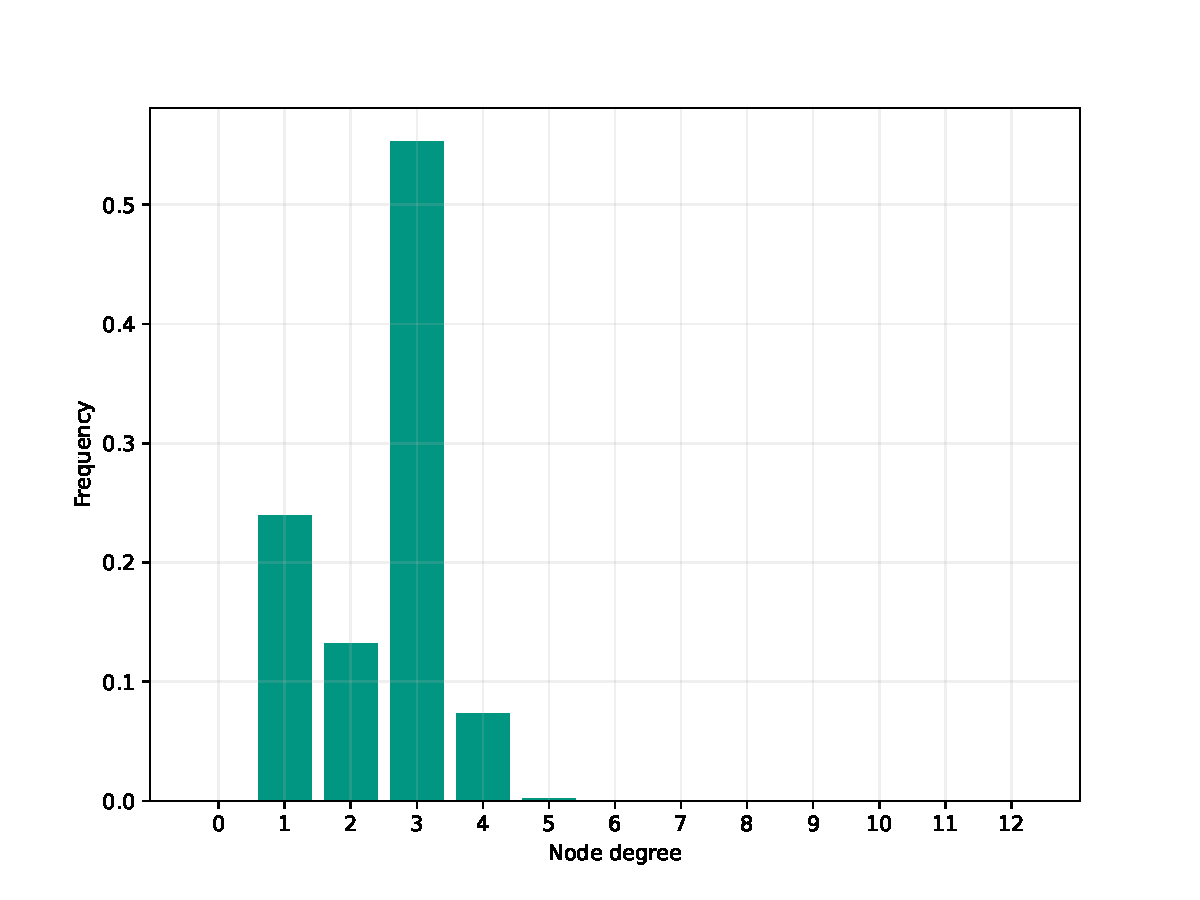
\includegraphics[width=0.6\linewidth]{graphics/degree_overview_europe.pdf}
    \caption{Degree distribution of the PTV Europe road network. The x-axis represents the vertex degree, and the y-axis shows the fraction of vertices with that degree. A single node with degree 12 has the highest degree.}
    \label{fig:degree_dist_europe}
\end{figure}

To examine whether this low average degree alone is sufficient to yield small separators, we generate connected random graphs matching this average degree.
The generation process involves two main steps.
First, a random spanning tree is created for a given set of \(n\) vertices using the algorithm described by Broder \cite{broder_generating_1989}.
This algorithm performs a random walk starting from an arbitrary vertex on the complete graph of \(n\) vertices.
An edge becomes part of the spanning tree the first time a vertex is discovered via that edge during the walk.
The process continues until all vertices are visited, resulting in a uniformly sampled random spanning tree in expected time \bigO{n \log n}.

It is noteworthy that random trees generated in this manner exhibit properties distinct from those of road networks.
For instance, the diameter of such random trees is known to be in \bigO{n^{1/2}} \cite{chlamtac_tree-based_1987}.
This differs from empirical observations on road networks, such as subgraphs from the nested dissection of the Karlsruhe graph, where the diameter appears smaller, estimated empirically as \bigO{n^{0.3683}}.
This observed diameter growth is visualized in \cref{fig:diameter_karlsruhe}.

\begin{figure}[tbhp]
    \centering
    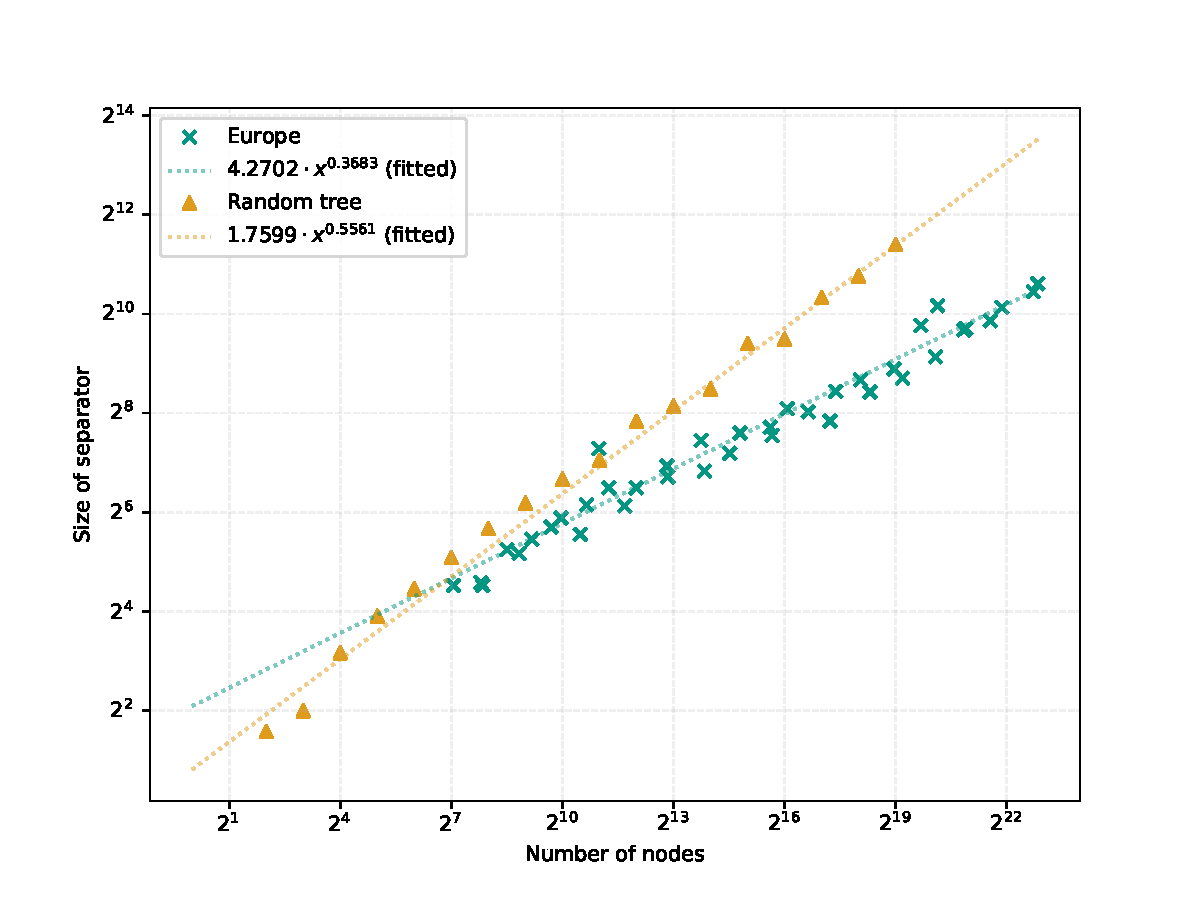
\includegraphics[width=0.6\linewidth]{graphics/diameters.pdf}
    \caption{Empirical diameter growth observed in the Karlsruhe road network subgraph. The plot shows the diameter (y-axis) as a function of the number of nodes \(n\) (x-axis, log scale).}
    \label{fig:diameter_karlsruhe}
\end{figure}

Following the generation of the initial random spanning tree, we proceed to the second step: adding edges randomly between pairs of non-adjacent vertices.
This edge addition continues until the target average degree of \(2.5\) is reached for the entire graph.
The resulting graphs, by construction, lack the inherent locality often present in road networks.
A consequence of adding these random edges is a notable decrease in the graph diameter.
For example, graphs generated with one million nodes using this method exhibit diameters of approximately 40.

These synthetic graphs do not replicate the small separator sizes observed in real-world road networks.
Experiments yielded large top-level separators, whose sizes scaled approximately linearly with the graph size \(n\), i.e., as \bigO{n}.
However, separators found during subsequent recursive partitioning behaved differently: their sizes were significantly smaller than this linear trend would predict for the corresponding subgraph sizes.
We attribute this deviation to structural changes in the subgraphs induced by the partitioning process.
Specifically, the large top-level separators often remove a significant fraction of the non-tree edges that were originally added to achieve the target average degree of approximately \(2.5\) in the parent graph.
Consequently, the resulting subgraphs become sparser—our observations showed a decrease in average degree to approximately \(2.2\)—and increasingly dominated by their underlying tree structure.
This shift means these subgraphs effectively belong to a different, more tree-like graph class than initially generated, which naturally leads to smaller relative separator sizes.
The separator scaling is illustrated in \cref{fig:same_degree}.



\begin{figure}[tbhp]
    \centering
    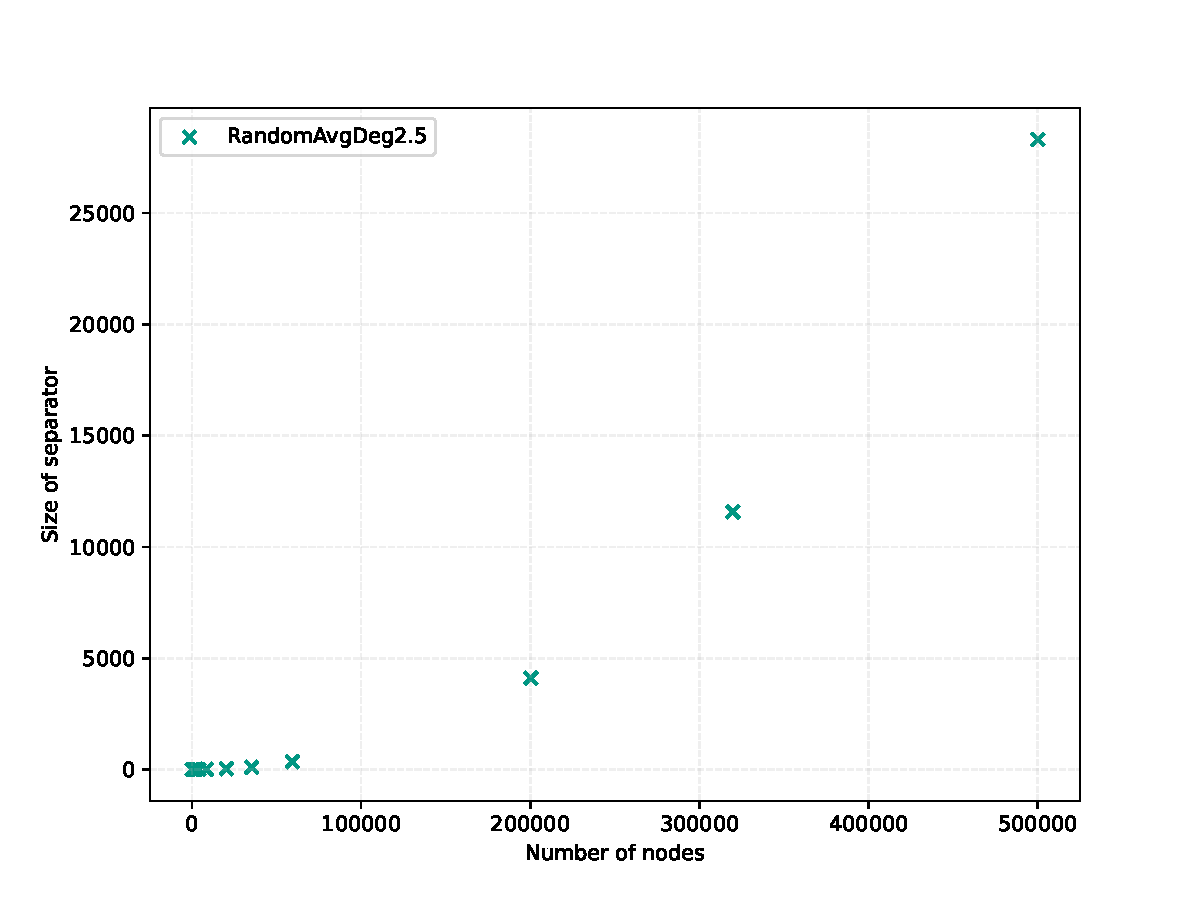
\includegraphics[width=0.6\linewidth]{graphics/RandomAvgDeg2.5.pdf}
    \caption{Separator sizes observed in random graphs generated with an average degree matching the PTV Europe road network (\( \approx 2.5 \)).}
    \label{fig:same_degree}
\end{figure}

We also conduct experiments generating graphs that match not just the average degree, but the specific degree distribution of the reference road network.
This involves a similar process of starting with a random tree and adding edges randomly.
However, edge addition is constrained: an edge \( (u, v) \) is added only if adding it does not cause either vertex \(u\) or \(v\) to exceed the count allocated for their respective degrees according to the target distribution sampled from the road network.
The results obtained from this refined approach are largely similar to those using only the average degree constraint.
It is important to note, however, that precisely replicating the target degree distribution using this generation process presents challenges.
While the maximum degree observed in the generated graphs generally approximately aligns with that of the reference road network, discrepancies arise in the distribution concerning nodes with higher degrees.
Specifically, the underlying structure of the initial random spanning tree tends to produce more vertices with high degrees compared to the road network.
Approximately 1.8\% of vertices in the random tree had a degree of 5 or greater, substantially more than the 0.2\% observed in the actual Europe dataset \cite{ptv_group_dimacs-europe_2009}.
Therefore, the process achieves an approximation of the target distribution rather than an exact match.
We contend, however, that this approximation is sufficiently close for the purposes of this investigation, and argue that the relatively small fraction of vertices whose degrees exceed the target constraints are unlikely to fundamentally alter the observed separator scaling behavior for this class of graphs.

The generated graphs continue to exhibit large separators, reinforcing the conclusion drawn from the average-degree matching experiments.
These findings suggest that the degree distribution alone is likely insufficient to explain the empirically observed small separators.
Nevertheless, the low average degree remains an important factor.
Intuitively, sparser graphs, possessing fewer edges overall, should generally be easier to partition compared to denser graphs.

\section{Locality}
\label{sec:synthetic:locality}

Building upon the previous experiments focused solely on degree distribution, we maintain the core methodology of first generating a random spanning tree and then augmenting it with additional edges to achieve a desired average degree.
The crucial difference in the approach detailed in this section lies in the edge augmentation phase: we introduce constraints intended to promote locality.
This modification reflects the inherent spatial structure of road networks, where connections predominantly link geographically proximate locations.
Two distinct strategies for introducing locality during edge addition are explored.

Our first approach attempts to simulate locality based on distances within the initial random spanning tree structure.
As before, we begin by generating a random spanning tree using Broder's algorithm \cite{broder_generating_1989}.
Subsequently, edges are added between non-adjacent vertices until a target average degree, chosen as \(2.5\) to approximate that of road networks, is achieved.
To incorporate locality, the probability of adding an edge between two vertices \(u\) and \(v\) is made dependent on their distance \( \text{dist}_T(u, v) \) within the initial spanning tree \(T\).
Specifically, we select a random vertex \(x\) and choose a second vertex \(y\) with a probability related to \(f(\text{dist}_T(x, y))\), where \(f\) is a decreasing function.

The computation of tree distances \(\text{dist}_T(x, y)\) for numerous candidate pairs \((x,y)\) is a critical step in this edge addition phase.
Initially, for each randomly selected vertex \(x\) and potential neighbor \(y\), we performed a Breadth-First Search (BFS) within the tree \(T\) to find \(\text{dist}_T(x, y)\).
While BFS on a tree is linear in the number of vertices \(n\), repeated invocations for many pairs proved computationally intensive for larger graphs.
To accelerate this, we adopted an approach based on Lowest Common Ancestor (LCA) queries.
This involved an initial precomputation of an LCA data structure for the tree \(T\), which can be achieved in \bigO{n \log n} time (e.g., using an Euler tour and sparse table for Range Minimum Queries, enabling \bigO{1} query time).
Once the LCA of two nodes \(u\) and \(v\) is known, their tree distance is given by \(\text{dist}_T(u, v) = \text{depth}(u) + \text{depth}(v) - 2 \cdot \text{depth}(lca(u,v))\).
Although a single BFS is also linear, this LCA-based method yielded a significant speedup, due to better parallelization.
Nevertheless, even with this optimization, the approach of potentially considering many \(y\) candidates for each \(x\) (full sampling) remained too slow for large graphs.
A possible further refinement, not explored in this work, could involve capping the search for \(y\) (e.g., limiting BFS depth or number of hops from \(x\)), under the assumption that for rapidly decaying probability functions \(f\), the likelihood of adding edges to very distant nodes becomes negligible.

Experiments using functions such as \( f(\text{dist}) = 1/\text{dist} \) result in graphs that still exhibit large separators scaling as \bigO{n}.
For subgraphs of the nested dissection we observe again the super-linear decrease in separator size, but the top-level separators remain large.
Using moderately decaying functions like \( f(\text{dist}) = 1/\text{dist}^2 \) leads to separators that scale sub-linearly but they are still significantly larger than \bigO{n^{1/3}}, especially the constant factor, where we are one to two orders of magnitude larger than the expected size, despite having the same average degree.
Conversely, using rapidly decaying functions like \( f(\text{dist}) = 2^{-\text{dist}} \) leads to separators of almost constant size, likely due to the graph structure remaining very close to the initial tree.

While the initial experiments using simple decay functions \(f(\text{dist}_T)\) did not yield the desired separator scaling, the concept of incorporating locality based on distances within the existing network structure (represented here by the initial tree) remains potentially insightful.
Such a metric might capture aspects beyond mere Euclidean distance, possibly relating to factors like travel time reduction incentives for new connections within the existing network topology.
However, our preliminary results indicated a high sensitivity to the choice of the decay function \(f\), with simple functional forms leading to either overly large or near-constant separator sizes.
Identifying a function capable of consistently producing \bigO{n^{1/3}} scaling appeared non-trivial and potentially specific to this particular generative model, lacking immediate theoretical guidance or clear real-world correspondence.
Given these initial findings and the decision to prioritize the investigation of other structural properties such as geometric locality, planarity, and explicit hierarchy, we opted not to pursue an exhaustive empirical search for an optimal tree-distance decay function within the scope of this work.

Our second approach incorporates geometric locality directly.
The core idea is to construct a graph starting with a basic connected structure and then augment it by adding only edges that connect geometrically close vertices, until a target average degree (e.g., \(2.5\)) is achieved.
To establish a meaningful threshold for 'closeness', we relate it to the natural scale derived from the spatial distribution of points.
Specifically, we first sample \(n\) points uniformly within a defined spatial domain (e.g., a circle).
We then compute the Minimum Spanning Tree (MST) of these points using Euclidean distances, via Kruskal's algorithm \cite{kruskal_shortest_1956}.
The maximum edge length found within this MST, denoted \(\ell_{\max}\), serves as our threshold distance, capturing a characteristic length scale of the initial sparse connection of the points.
The graph generation then proceeds by initially taking the edges of the MST.
Subsequently, additional edges \((u, v)\) between non-adjacent vertices are iteratively added, but crucially, only if their Euclidean distance is less than or equal to the threshold \(\ell_{\max}\).
This edge addition process continues until the overall graph reaches the target average degree of \(2.5\).
For efficient implementation of the edge addition step, we utilize spatial queries: for a randomly selected vertex \(u\), we query for potential neighbors \(v\) within the radius \(\ell_{\max}\) and randomly select one to connect to, avoiding multi-edges and self-loops.

Despite incorporating this explicit geometric constraint, the resulting synthetic graphs fail to exhibit the desired small separator sizes characteristic of road networks.
To analyze the separator properties of these graphs, we computed recursive separators.
Implementations from both IntertialFlowCutter and KaHIP were utilized for this purpose.
Our experiments using these methods indicate that separators in these geometrically generated graphs scale approximately as \bigO{n^{1/2}}.
This outcome is visualized in \cref{fig:geometric_locality_separators}.

\begin{figure}[tbhp]
    \begin{subfigure}{0.35\linewidth}
        \centering
        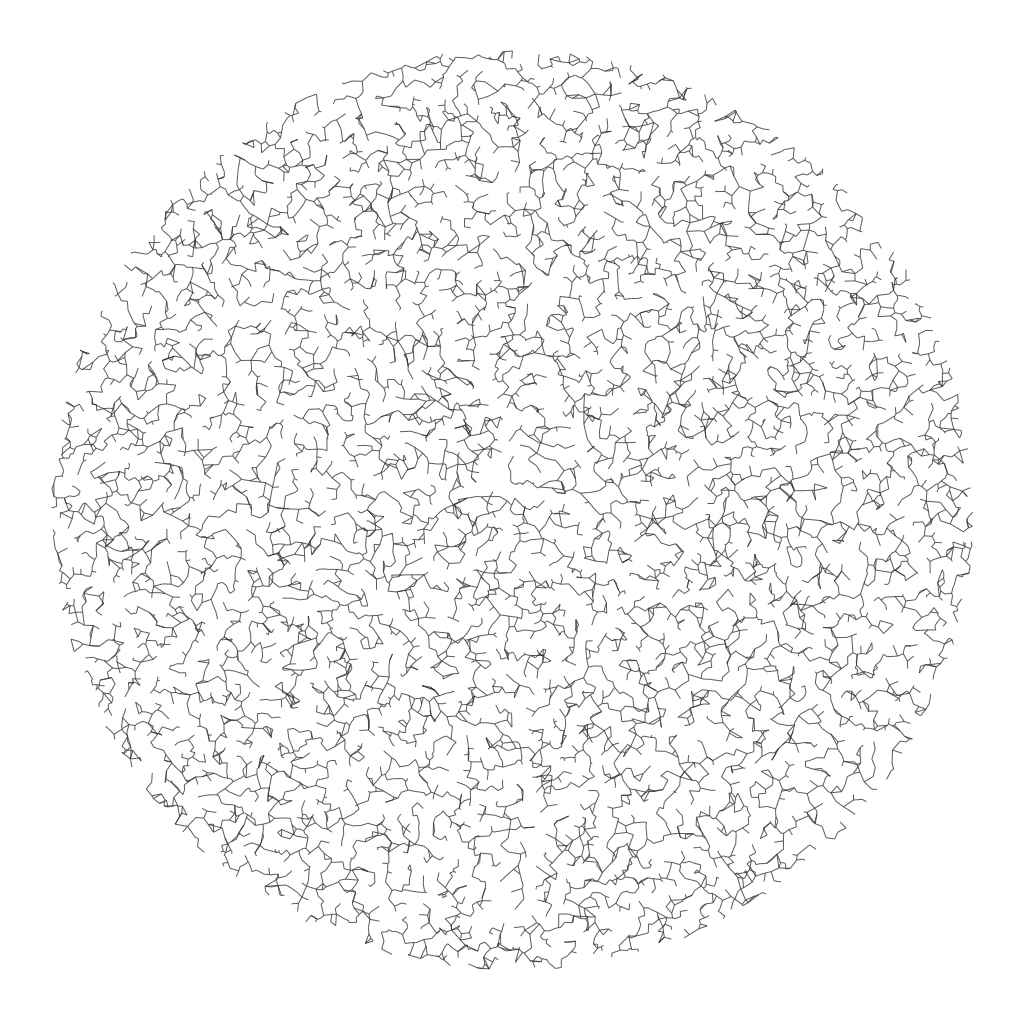
\includegraphics[width=\linewidth]{graphics/local_embedding.png}
        \caption{Visualization of a graph with 10K nodes generated using the geometric locality method.}
        \label{fig:geometric_locality_graph_viz}
    \end{subfigure}
    \hfill
    \begin{subfigure}{0.55\linewidth}
        \centering
        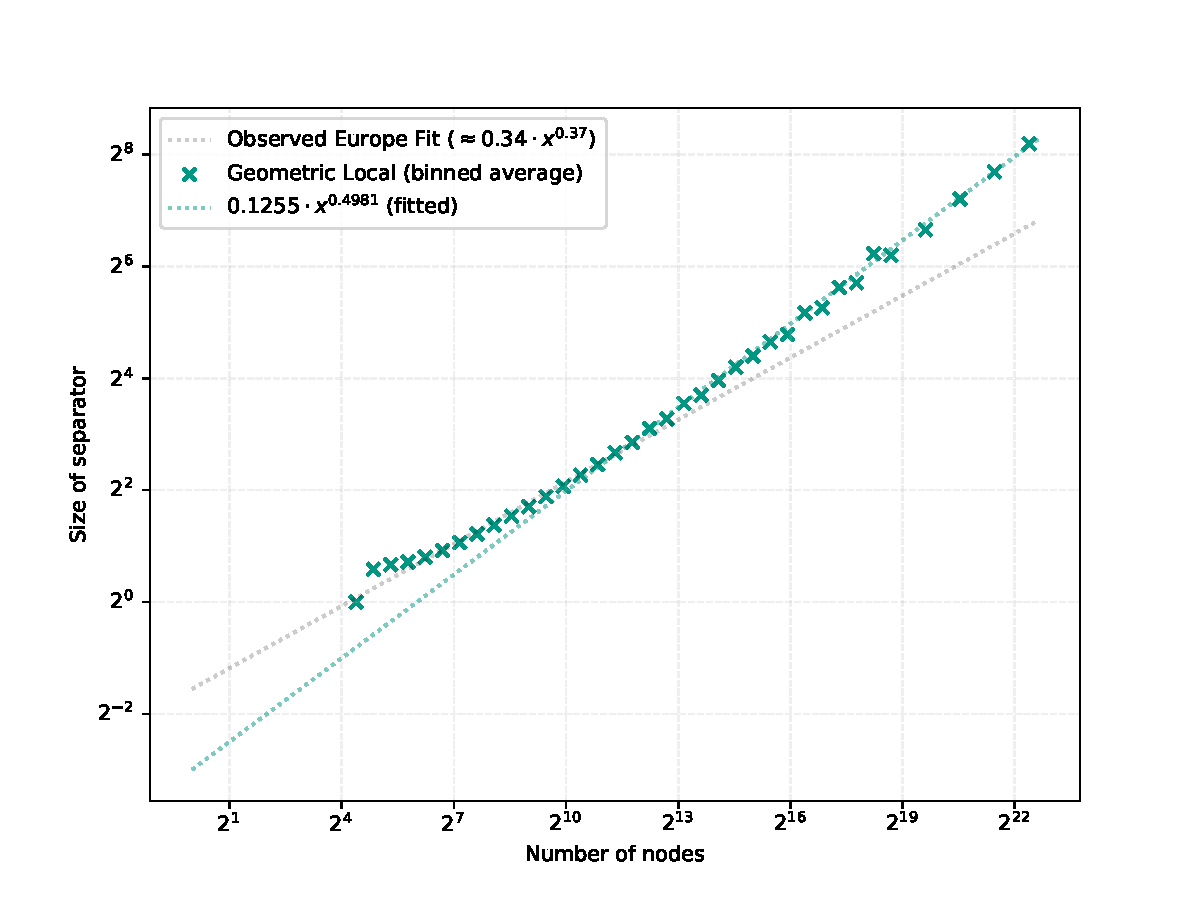
\includegraphics[width=\linewidth]{graphics/sep_local_embedding.pdf}
        \caption{Separator size scaling for synthetic graphs generated with geometric locality. The fit shown excludes subgraphs with \( \le 1000 \) vertices due to their disproportionately large separatos. }
        \label{fig:geometric_locality_sep_plot}
    \end{subfigure}
    \caption{Synthetic graph generation using geometric locality and analysis of separator sizes. }
    \label{fig:geometric_locality_separators}
\end{figure}

The results from the geometric locality approach suggest that merely combining low average degree with this specific form of locality is insufficient to reproduce the cubic root separator sizes of road networks.

\paragraph{Real-World Implications}

It is worth considering the practical implications of different asymptotic growth rates for separator sizes within the typical scale of road networks.
While \bigO{c_1\cdot n^{1/3}} and \bigO{c_2 \cdot n^{1/2}}, with \(c_2 \ll c1\), diverge for large \(n\), the actual separator sizes for graphs up to around 20 million vertices are similar.
The performance of algorithms leveraging graph separators in real-world applications may be more influenced by the absolute sizes of separators achievable in practice, compared to a specific scaling model.
Performance gains, for example for CCH \cite{dibbelt_customizable_2016}, could potentially be realized even if the separators behave like \(c \cdot n^{1/2}\) for a sufficiently small \(c\), as the absolute separator sizes remain manageable for networks of practical relevance.

\paragraph{Initial Deviations in Separator Scaling}

An interesting characteristic is observable for graphs with small node counts in empirical studies of road networks.
As a careful reader may notice in \cref{fig:separator_size_loglog_non_binned}, real road networks often exhibit a deviation in separator scaling for graphs containing approximately \(2^6\) nodes.
\cref{fig:outlier_histograms} presents histogram plots to better visualize the prevalence of these instances for both real-world data and our synthetic model.
Specifically, \cref{fig:real_europe_hist} shows this phenomenon for European road network samples.
These plots reveal an initial peak in relative separator size for small graphs, followed by a slight decrease, before the data align with the more dominant scaling trend observed for larger graphs.

\begin{figure}[tbhp]
    \centering
    \begin{subfigure}{0.48\linewidth}
        \centering
        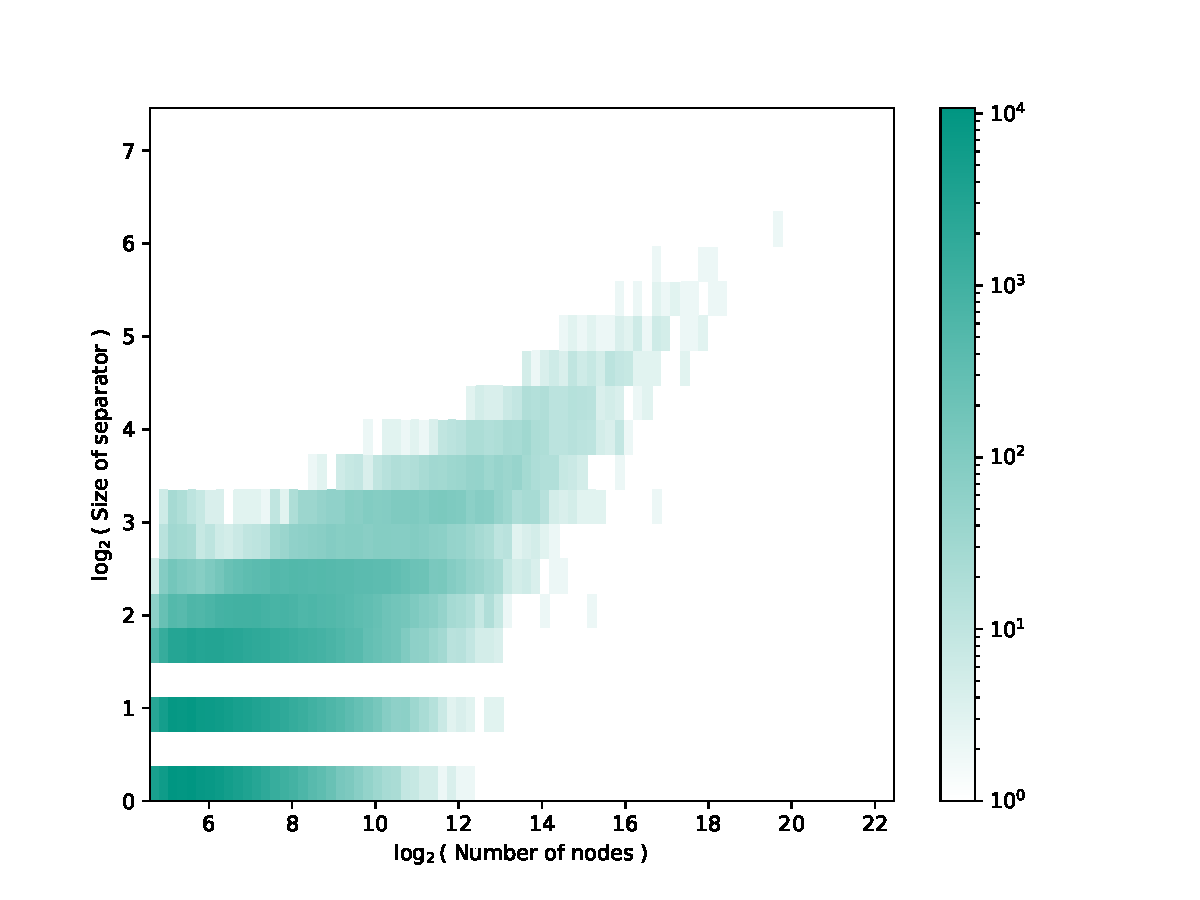
\includegraphics[width=\linewidth]{graphics/Germany-hist.pdf}
        \caption{Histogram of separator sizes for the European road network.}
        \label{fig:real_europe_hist}
    \end{subfigure}
    \hfill
    \begin{subfigure}{0.48\linewidth}
        \centering
        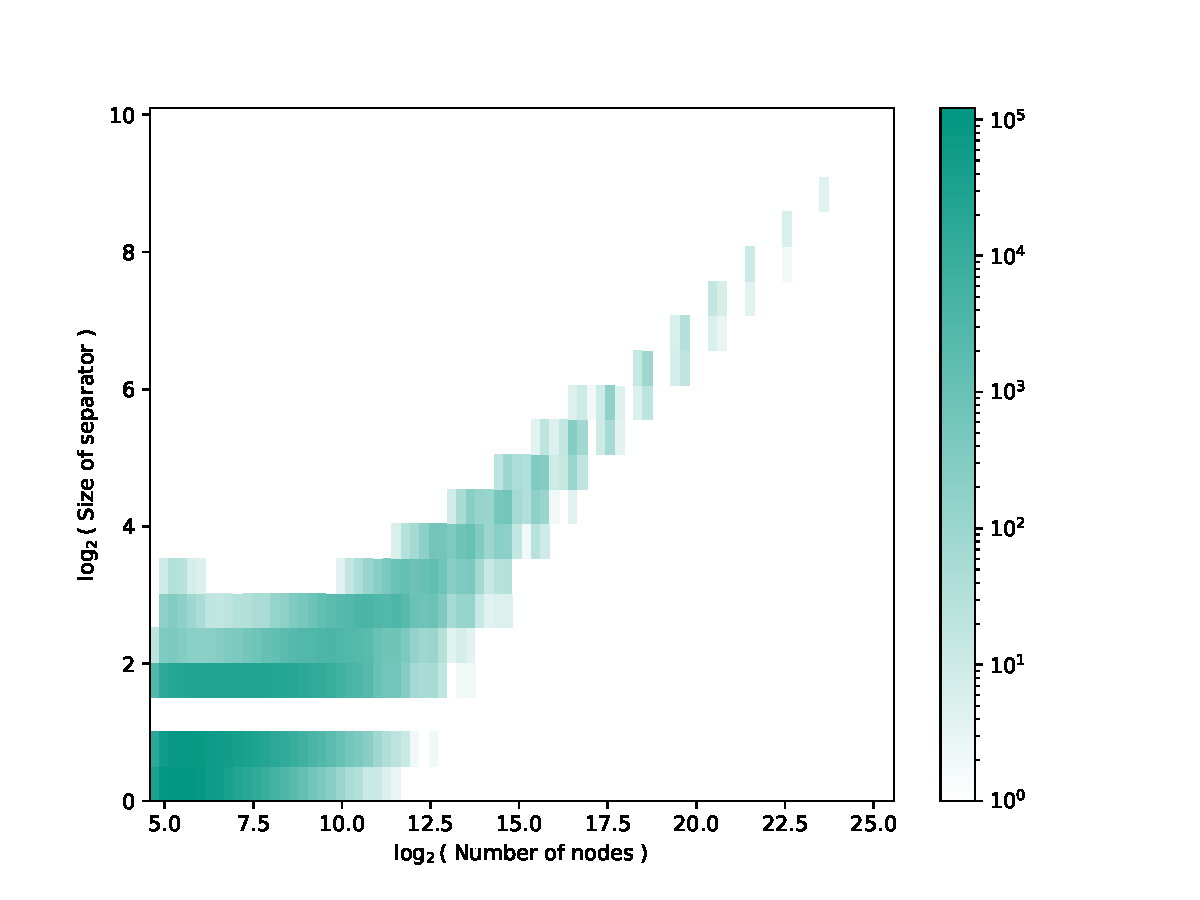
\includegraphics[width=\linewidth]{graphics/local_embedding-hist.pdf}
        \caption{Histogram of separator sizes for synthetic graphs using geometric locality.  }
        \label{fig:local_embedding_hist}
    \end{subfigure}
    \caption{Histograms illustrating the distribution of separator sizes, comparing real road networks (left) and the geometric locality model (right). A slight increase in separator size is observed for graphs with \(\approx 2^6\) nodes.}
    \label{fig:outlier_histograms}
\end{figure}

Our synthetic graphs generated using the geometric locality approach exhibit a similar initial pattern, as can be discerned from the histogram in \cref{fig:local_embedding_hist}.
This initial behavior in the synthetic model appears qualitatively comparable, although slightly more pronounced than in the real network data.
This correspondence is noteworthy.
It suggests that the geometric locality model, despite failing to replicate the overall asymptotic separator scaling of \bigO{n^{1/3}}, may capture certain structural properties relevant at smaller graph scales that are present in actual road networks.

\section{Planarity}
\label{sec:synthetic:planarity}

We examine separator properties in two classes of planar graphs: grids and Delaunay triangulations.
These serve as fundamental theoretical models for planar structures relevant to the study of road networks due to their near-planarity.
In our study, these graph classes are sparsified to achieve a low average degree (approximately \(2.5\)), reflecting the sparsity observed in road networks.

Our initial investigation focuses on grid graphs, a fundamental class known to possess separators scaling as \bigO{n^{1/2}}.
To align their sparsity with road networks, we generate modified grids with an average degree of approximately \(2.5\).
The generation process starts with a square two-dimensional grid graph.
Edges are then removed uniformly at random until the target average degree is reached over the entire graph.
Subsequently, we identify and utilize the largest connected component for analysis.
We observe that even without explicit mechanisms to prevent disconnection during edge removal, the largest connected component typically encompasses a large fraction of the initial vertices.

Analysis of these sparse grid graphs reveals separator sizes consistent with the \bigO{n^{1/2}} asymptotic behavior of complete grids.
However, the constant factor associated with this scaling appears to be relatively small.
Consequently, although the asymptotic limit behavior differs from the \bigO{n^{1/3}} scaling empirically observed for road networks, the absolute separator sizes in these sparse grids are numerically similar to those of road networks for graphs up to typical sizes (e.g., around 20 million nodes).
This finding highlights that sparsity, even within a simple planar structure like a grid, can lead to separators that are small in absolute terms for practical graph dimensions.
\Cref{fig:sparse_grid_separators} illustrates a sample sparse grid and the observed separator scaling.

\begin{figure}[tbhp]
    \centering
    \begin{subfigure}{0.35\linewidth}
        \centering
        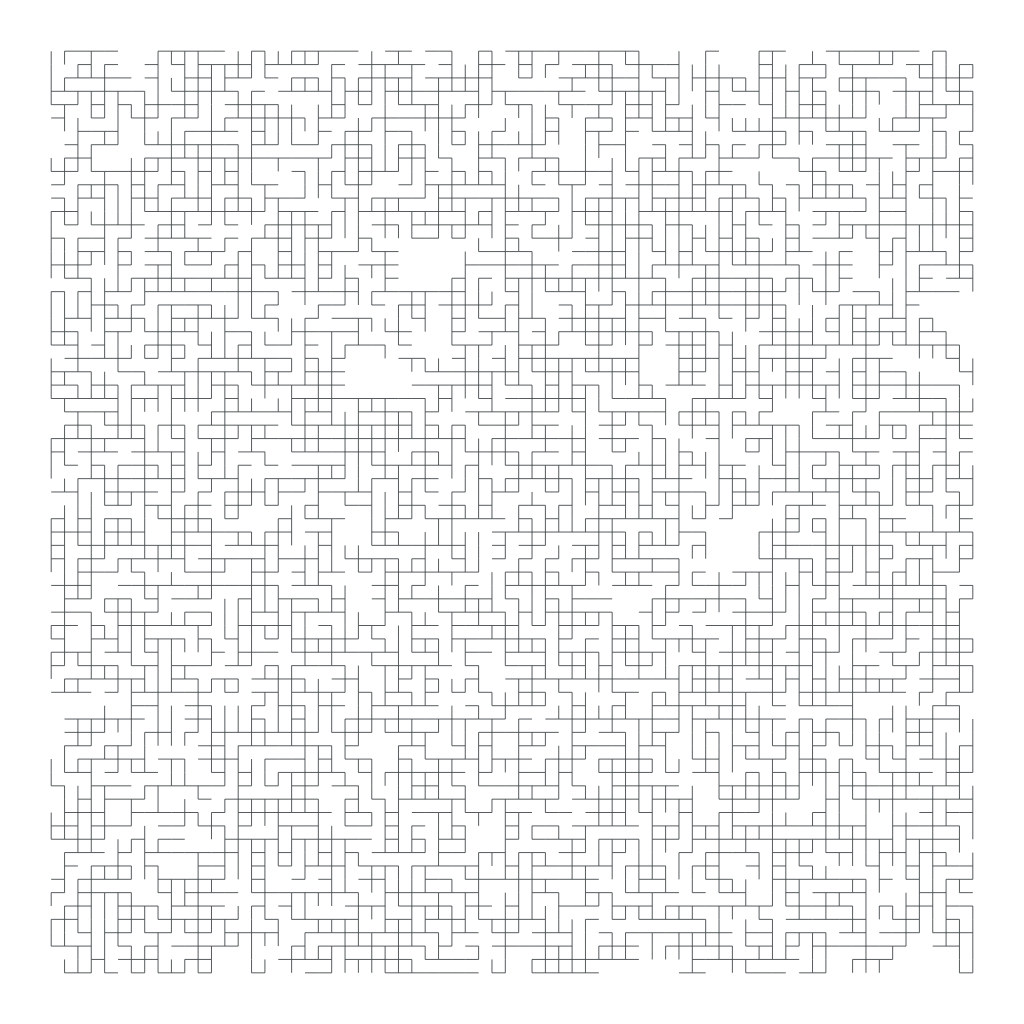
\includegraphics[width=\linewidth]{graphics/grid_avg_deg.png}
        \caption{Visualization of the largest connected component of a grid graph with \(\approx 10\text{K}\) nodes after random edge removal to achieve an average degree of \(2.5\).}
        \label{fig:sparse_grid_viz}
    \end{subfigure}
    \hfill
    \begin{subfigure}{0.55\linewidth}
        \centering
        \includegraphics[width=\linewidth]{graphics/sep_grid_avg_deg.png}
        \caption{Separator size scaling for sparse grid graphs (average degree \(2.5\)). Separator sizes scale approximately as \bigO{n^{1/2}}, but with a small constant factor leading to absolute sizes comparable to road networks at practical scales. The fit shown excludes subgraphs with \( \le 1000 \) vertices due to their disproportionately large separators.}
        \label{fig:sparse_grid_sep_plot}
    \end{subfigure}
    \caption{Analysis of sparse grid graphs with average degree \(2.5\).}
    \label{fig:sparse_grid_separators}
\end{figure}

We extend this investigation to Delaunay triangulations, which can be viewed as a generalization of grids derived from point sets.
Our process involves sampling points uniformly at random in a two-dimensional space and computing their Delaunay triangulation.
Similar to the grid experiments, we then randomly delete edges from the triangulation until the average degree reaches the target value of \(2.5\), again analyzing the largest connected component.

As might be expected, the results obtained from these sparse Delaunay graphs are largely analogous to those from sparse grids.
The separators exhibit scaling consistent with \bigO{n^{1/2}}, characteristic of planar graphs, yet the associated constant factors are small.
This again leads to absolute separator sizes that are numerically comparable to those measured in road networks for graphs of relevant sizes.
These findings are depicted in \cref{fig:sparse_delaunay_separators}.

\begin{figure}[tbhp]
    \centering
    \begin{subfigure}{0.35\linewidth}
        \centering
        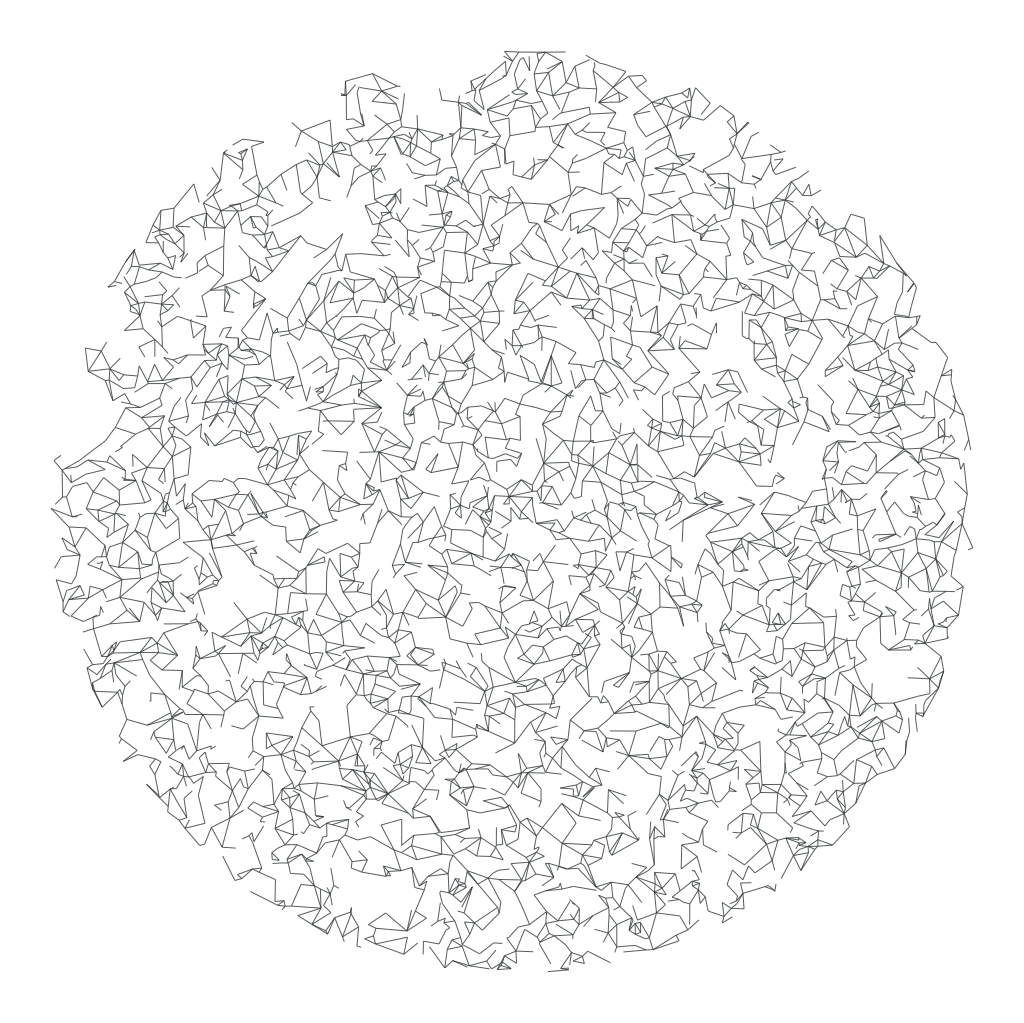
\includegraphics[width=\linewidth]{graphics/delaunay_avg_deg.png}
        \caption{Visualization of a sparse Delaunay triangulation with 5K nodes after random edge removal to achieve an average degree of \(2.5\).}
        \label{fig:sparse_delaunay_viz}
    \end{subfigure}
    \hfill
    \begin{subfigure}{0.55\linewidth}
        \centering
        \includegraphics[width=\linewidth]{graphics/sep_delaunay_avg_deg.png}
        \caption{Separator size scaling for sparse Delaunay graphs (average degree \(2.5\)). Separator sizes scale approximately as \bigO{n^{1/2}} with small constant factors, yielding absolute sizes similar to road networks at practical scales. The fit shown excludes subgraphs with \( \le 1000 \) vertices due to their disproportionately large separatos.}
        \label{fig:sparse_delaunay_sep_plot}
    \end{subfigure}
    \caption{Analysis of sparse Delaunay graphs with average degree \(2.5\).}
    \label{fig:sparse_delaunay_separators}
\end{figure}

The experiments with sparse grids and Delaunay triangulations suggest that combining geometry with low average degree results in graphs whose practical separator sizes are close to those of road networks, despite differing asymptotic scaling.

\section{Highway Dimension}
\label{sec:synthetic:highway_dimension}

Given that the simpler graph models explored in previous sections do not reproduce the observed \bigO{n^{1/3}} separator scaling of road networks, we turn our attention to more complex generative processes designed to capture other relevant structural properties.
One such property is highway dimension, introduced by Abraham et al. \cite{abraham_highway_2010}.
Intuitively, a graph possesses a small highway dimension if, for every radius \(r > 0\), there exists a sparse set of vertices \(S_r\) such that every shortest path longer than \(r\) intersects \(S_r\).
A set is considered sparse if every ball of radius \(\mathcal{O}(r)\) contains only a small number of vertices from \(S_r\) \cite{abraham_highway_2010}.
The significance of this property stems from the finding that low highway dimension provides provable performance guarantees for several important route planning algorithms, including REACH \cite{goldberg_reach_2006}, Contraction Hierarchies \cite{geisberger_contraction_2008}, Highway Hierarchies \cite{sanders_highway_2005}, Transit Node Routing \cite{bast_fast_2007}, and SHARC \cite{bauer_sharc_2010}.

The work introducing highway dimension also proposes a synthetic graph generator (henceforth ABR generator) intended to produce graphs exhibiting this property \cite{abraham_highway_2010}.
A good explanation of the generation process is provided in \cite{hutchison_synthetic_2010}, which we summarize here.
The generation process operates iteratively.
It begins with an empty graph \( G = (V, E) = (\emptyset, \emptyset) \) and progressively adds new vertices \(v_t\) to \(V\), whose locations in the metric space are chosen randomly.
Throughout this process, the generator maintains a series of \(2^i\)-covers, denoted \(C_i\), for each level \(i\) where \(1 \leq i \leq \log D\), and \(D\) represents the diameter of the metric space.
A set \(C_i \subseteq V\) is a \(2^i\)-cover if any two vertices \(u, v \in C_i\) satisfy \(d(u, v) \geq 2^i\), and every vertex \(u \in V\) is within distance \(2^i\) of some vertex in \(C_i\).
When a new vertex \(v_t\) is added, the generator identifies the smallest index \(i\) such that there exists a vertex \(w \in C_i\) with \(d(v_t, w) \leq 2^i\).
The new vertex \(v_t\) is then added to all covers \(C_j\) for which \(0 \leq j < i\).
If no such index \(i\) exists, \(v_t\) is added to all cover sets \(C_j\).
Edges are subsequently added based on these covers and a tuning parameter \(k\).
For each cover \(C_j\) containing \(v_t\) (where \(0 \leq j < i\)), and for each existing vertex \(w \in C_j\), an edge \((w, v_t)\) is added if their distance satisfies \(d(w, v_t) \leq k \cdot 2^j\).
Furthermore, for each \(C_j\) containing \(v_t\) where \(j < \log D\) and \(v_t\) is also present in \(C_{j+1}\), an edge is added connecting \(v_t\) to its nearest neighbor within the set \(C_{j+1}\).
For our experiments, we adopt parameter settings similar to those used by \cite{hutchison_synthetic_2010}, setting the diameter \(D = 2^{25}\) and the connection parameter \(k = \sqrt{2}\).

Bauer et al. also describe an alternative node sampling strategy aimed at creating structures resembling city clusters \cite{hutchison_synthetic_2010}.
We implement and test both the uniform random sampling and this cluster-based sampling approach.
Our experiments indicate no significant difference in the resulting separator sizes between the two sampling methods using the ABR generator framework.

The analysis of graphs generated using the ABR method yields separators that scale approximately as \bigO{n^{1/2}}.
This result is noteworthy because graphs generated by this process are typically highly non-planar.
It serves as a reminder that observing \bigO{n^{1/2}} separator scaling does not necessarily imply planarity.
\Cref{fig:abr_graph_separators} provides a visual example of an ABR-generated graph and illustrates the observed separator scaling.

\begin{figure}[tbhp]
    \centering
    \begin{subfigure}{0.35\linewidth}
        \centering
        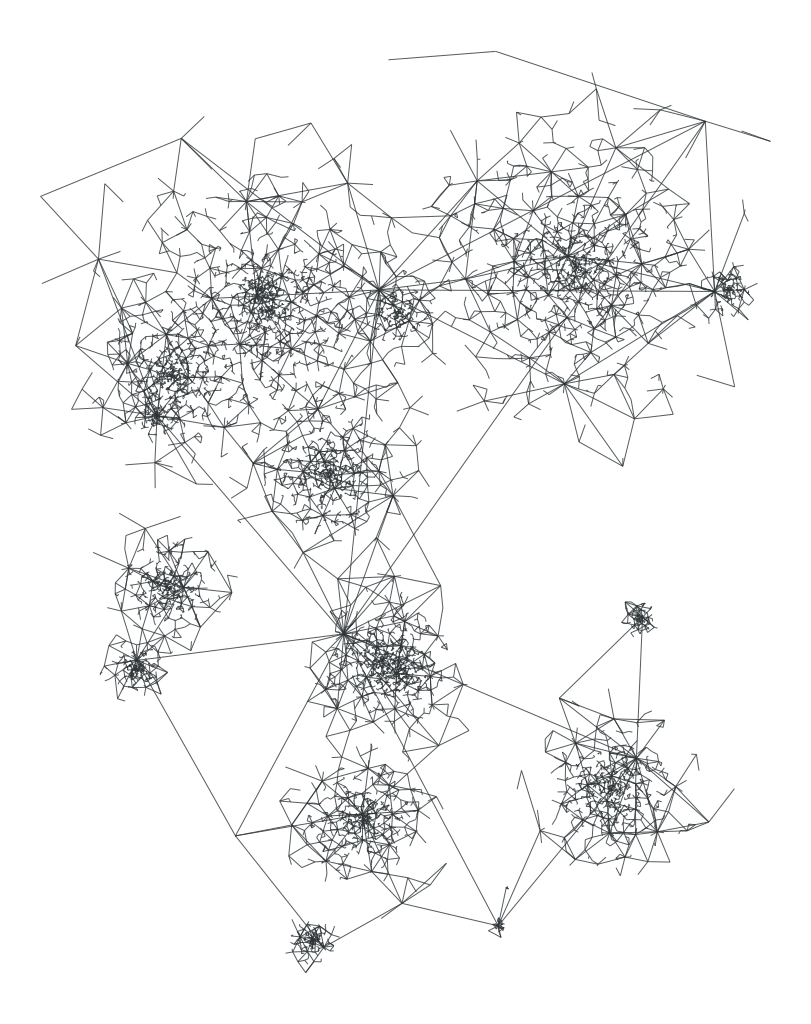
\includegraphics[height=\linewidth, angle=90]{graphics/highway.png}
        \caption{Visualization of a synthetic graph generated using the ABR low highway dimension algorithm with 10K nodes.}
        \label{fig:abr_graph_viz}
    \end{subfigure}
    \hfill
    \begin{subfigure}{0.55\linewidth}
        \centering
        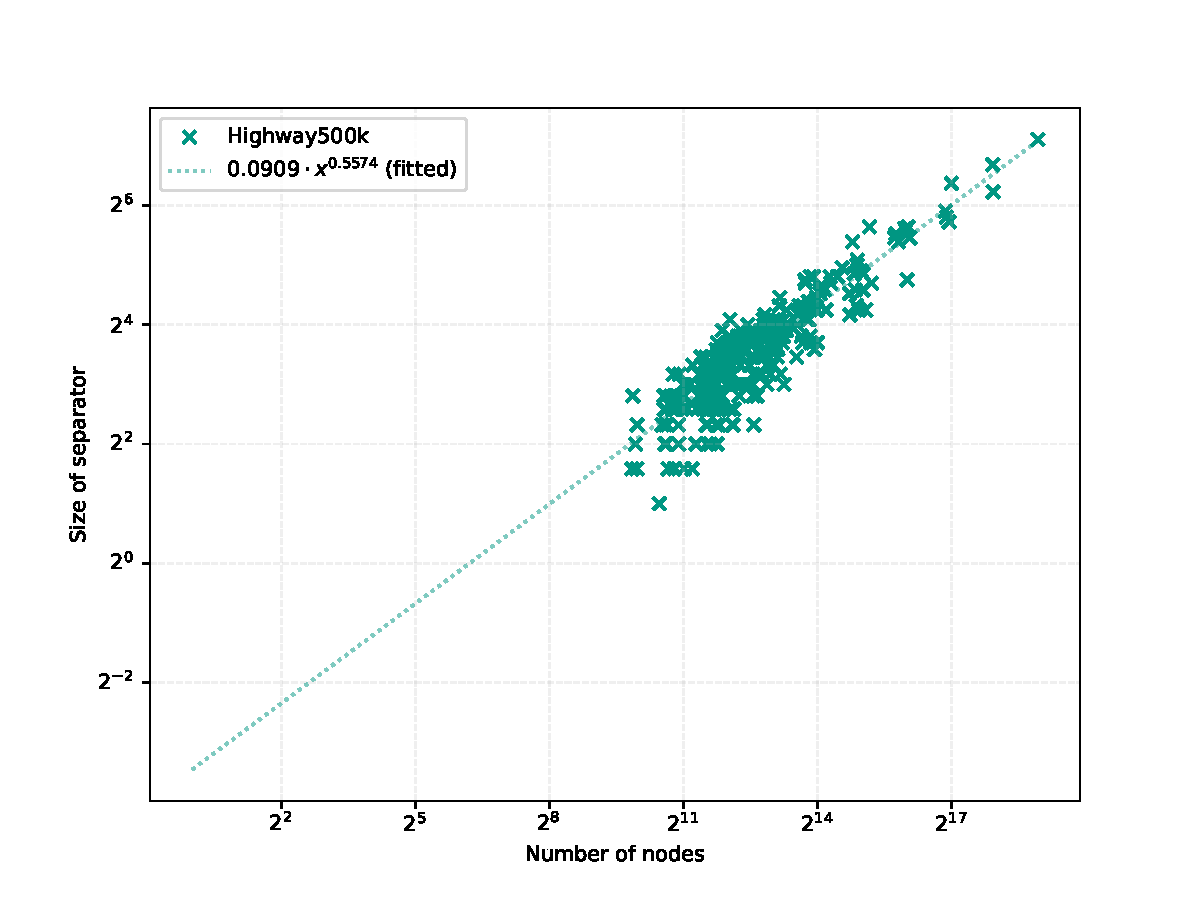
\includegraphics[width=\linewidth]{graphics/sep_highway.pdf}
        \caption{Separator size scaling observed during recursive partitioning of ABR-generated graphs. Separator sizes scale approximately as \bigO{n^{1/2}}. The fit shown excludes subgraphs with \( \le 256 \) vertices due to their disproportionately large separatos.}
        \label{fig:abr_graph_sep_plot}
    \end{subfigure}
    \caption{Analysis of synthetic graphs generated using the ABR algorithm \cite{abraham_highway_2010}.}
    \label{fig:abr_graph_separators}
\end{figure}

\section{Hierarchical Structure}

Real-world road networks intrinsically possess a hierarchical structure.
Different types of roads cater to different travel distances and volumes, forming levels within the network.
Depending on the specific taxonomy used, road networks are categorized into various numbers of classes or levels.
For instance, a common classification for Germany includes (using original German terms alongside translations):

\begin{itemize}
    \item Federal Motorways (Bundesautobahnen)
    \item Federal Highways (Bundesstraßen)
    \item State Roads (Landesstraßen)
    \item District Roads (Kreisstraßen)
    \item Municipal Roads (Gemeindestraßen)
\end{itemize}

This inherent hierarchy is another potentially relevant feature influencing separator sizes, which we investigate using synthetic models.

\subsection{Voronoi-Based Hierarchical Generator}

One approach to generating synthetic networks with hierarchical features follows the method proposed by Bauer et al. \cite{hutchison_synthetic_2010}.
This method utilizes Voronoi diagrams iteratively.
A Voronoi diagram, given a set of points \(P\), partitions the plane into convex regions, where each region contains the area closer to one point in \(P\) than to any other point in \(P\).
The generation process commences within a predefined initial polygon, which defines the spatial extent of the synthetic network.
Points, designated as sites \(P\), are then generated within this polygon according to a chosen sampling strategy.
One strategy involves sampling a specified number of points uniformly at random throughout the polygon's interior.
Alternatively, to better emulate settlement patterns, a clustered sampling approach can be employed.
This approach involves first sampling locations for a number of population centers within the polygon.
Each center is then assigned characteristics, such as a population size or an influence radius, drawn from a chosen distribution.
Subsequently, points are sampled in the vicinity of each city center, concentrated within its influence radius, with the number of points related to the city's size.

Regardless of the sampling method, the resulting set of points \(P\) serves as the input for computing the Voronoi diagram for this initial level.
The Voronoi diagram partitions the polygon into regions based on nearest-neighbor relationships to the points in \(P\).
The edges of this Voronoi diagram (where adjacent regions meet) are then added to the synthetic graph.
To introduce hierarchy, some of the resulting Voronoi regions (polygons) are selected, and the process is recursively applied within them: new points are sampled inside the selected region (using either uniform or clustered sampling), and a new Voronoi diagram is constructed within its boundaries, adding further edges to the graph.

Phase two of the generation process addresses the density of the graph \(G\) resulting from the Voronoi tessellation by constructing a sparse graph \(t\)-spanner \(H\).
A subgraph \(H\) is a \(t\)-spanner of \(G\) if it preserves all pairwise distances up to a multiplicative factor of \(t\).
The spanner is built using a greedy algorithm that iterates through the edges of \(G\) sorted by non-increasing length (longest first).
An edge \((u, v)\) with length \(len(u, v)\) is added to the spanner \(H\) only if the current shortest path distance between \(u\) and \(v\) within \(H\), denoted \(dist_H(u, v)\), is greater than \(t \cdot len(u, v)\).
To compute \(dist_H(u, v)\), Dijkstra's algorithm is employed.
Additionally, a union-find data structure maintains the connected components of \(H\), allowing for immediate addition of edges connecting previously disconnected vertices.
Bauer et al. propose processing edges in non-increasing order (longest first) as a heuristic primarily intended to improve the computational efficiency of the spanner construction; the idea is to handle long edges while the intermediate spanner graph \(H\) is still sparse, potentially speeding up distance computations \cite{hutchison_synthetic_2010}.
In our own experiments, however, we explore alternative edge processing orders.
We observe that processing the edges in a random order, or even in increasing order of length (shortest first), appears to produce graph structures with greater visual resemblance to actual road networks compared to the longest-first approach described by Bauer et al., without substantially increasing computation times in our experiments.

This generation method introduces artifacts.
For example, connections between major structures defined at higher levels (like large "cities") might be unrealistically sparse, potentially consisting of only a few edges.
Another artifact is that higher-level Voronoi edges (e.g., "highways" separating major regions) act as hard boundaries that lower-level edges (within regions) often do not cross, creating unrealistically effective separators along these top-level edges.

Analyzing separators in the final sparse graphs generated by this Voronoi-based method reveals interesting characteristics related to the hierarchy.
Plots of separator size versus subgraph size often exhibit noticeable local minima, which appear to correspond to the transitions between the hierarchical layers created during generation.
This can lead to separators of approximately constant size when partitioning cuts primarily occur between these major structures at layer intersections.
Within a single layer generated by the Voronoi tessellation (before sparsification), the separators tend to exhibit scaling closer to \bigO{n^{1/2}}.
Consequently, if the recursion depth is limited and the highest-level structures are allowed to grow large, their \bigO{n^{1/2}} separator behavior will dominate the separator size scaling.
\Cref{fig:voronoi_hierarchy} illustrates the structure and separator behavior of the final sparse graph.

\begin{figure}[tbhp]
    \centering
    \begin{subfigure}{0.35\linewidth}
        \centering
        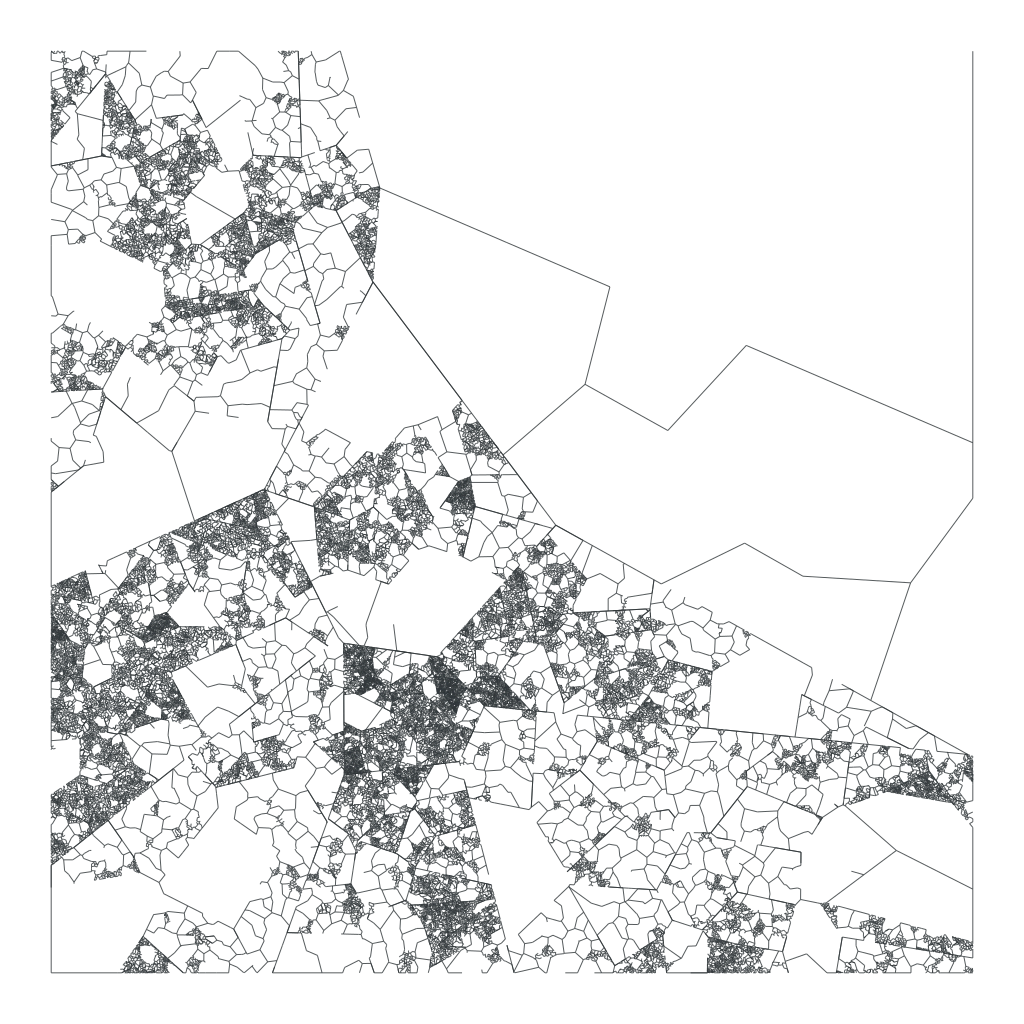
\includegraphics[width=\linewidth]{graphics/voronoi.png}
        \caption{Visualization of a synthetic graph generated using the Voronoi method.}
        \label{fig:voronoi_hierarchy_viz}
    \end{subfigure}
    \hfill
    \begin{subfigure}{0.55\linewidth}
        \centering
        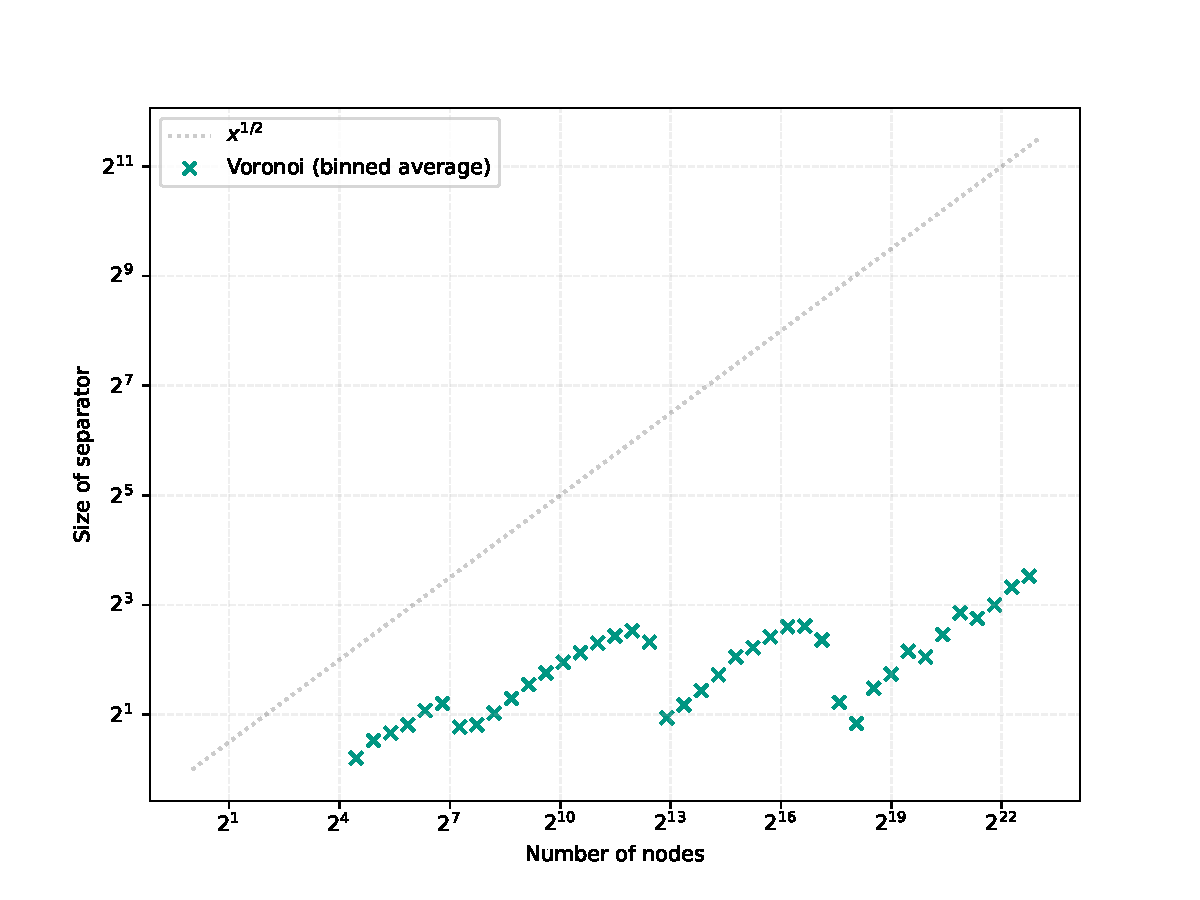
\includegraphics[width=\linewidth]{graphics/sep-voronoi.pdf}
        \caption{Separator size scaling for the hierarchical Voronoi graph, showing local minima at layer transitions.}
        \label{fig:voronoi_hierarchy_sep_plot}
    \end{subfigure}
    \caption{Analysis of synthetic graphs generated using the hierarchical Voronoi approach from Bauer et al. \cite{hutchison_synthetic_2010}.}
    \label{fig:voronoi_hierarchy}
\end{figure}

\subsection{Nested Grids}

To explore hierarchical effects in a more controlled manner, we also investigate a simpler but conceptually related approach using nested grids.
This method aims to construct a hierarchical graph by recursively embedding grid graphs within the cells of a parent grid, potentially allowing us to deliberately engineer specific separator scaling properties.
The fundamental idea involves placing copies of a subgraph (e.g., a square grid) into selected cells of a higher-level grid.
This resulting composite graph can then itself be treated as a subgraph to be placed within cells of a grid at an even higher level, and so on.
\cref{fig:nested_grid_analysis} shows a small conceptual example of a nested grid with three layers.

\begin{figure}[tbhp]
    \centering
    \begin{subfigure}{0.35\linewidth}
        \centering
        \includegraphics[width=\linewidth]{graphics/nestedgrid.pdf}
        \caption{Conceptual illustration of a simple nested grid structure with three hierarchical levels.}
        \label{fig:nested_grid_viz}
    \end{subfigure}
    \hfill
    \begin{subfigure}{0.55\linewidth}
        \centering
        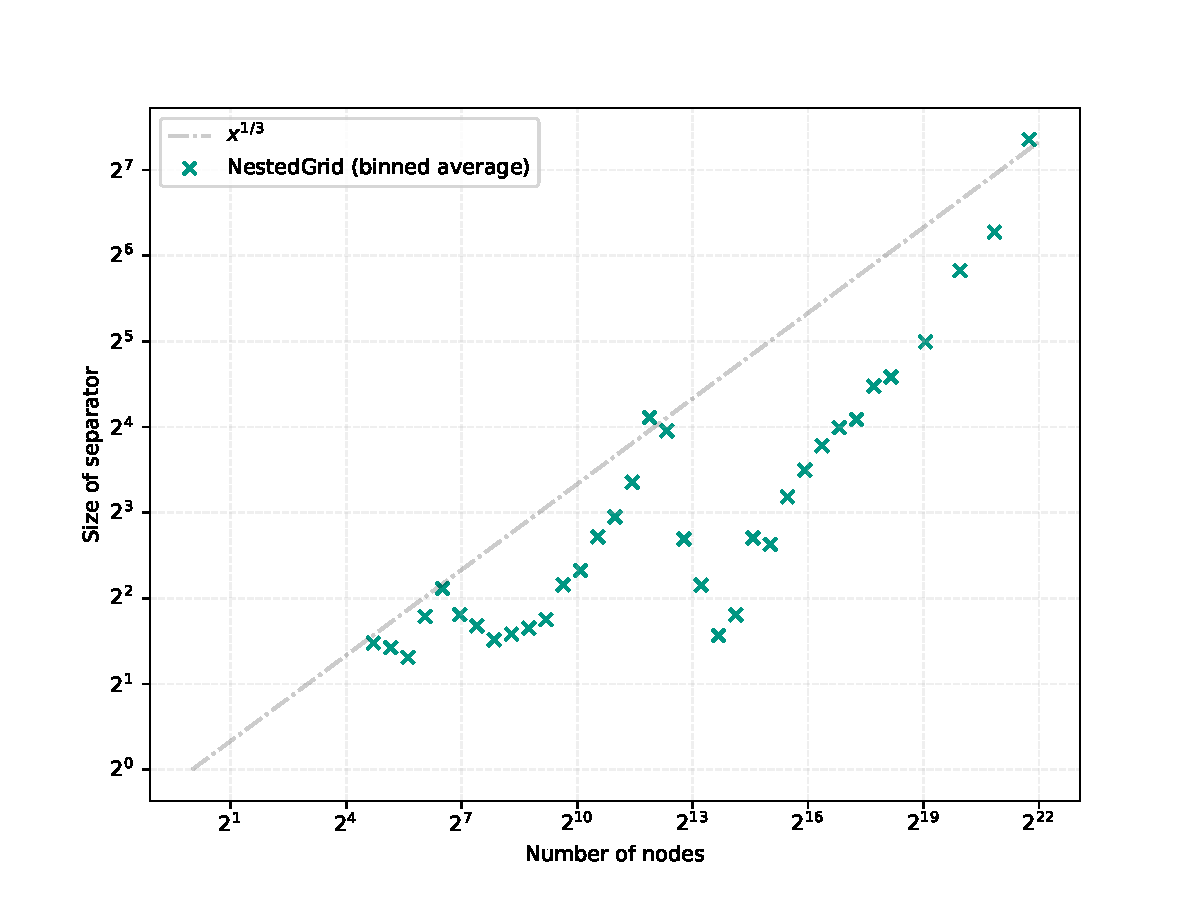
\includegraphics[width=\linewidth]{graphics/sep-nestedgrid.pdf}
        \caption{Separator size scaling for nested grids, showing pronounced local minima.}
        \label{fig:nested_grid_sep_plot}
    \end{subfigure}
    \caption{Analysis of synthetic graphs generated using the nested grid approach.}
    \label{fig:nested_grid_analysis}
\end{figure}

A nested grid construction with \(l\) layers is determined by \(l\) grid sizes (specifying the dimensions of the grid at each layer) and \(l-1\) placement parameters (specifying how many subgraphs from layer \(i+1\) are placed within layer \(i\)).
This parameterization offers the possibility of attempting to enforce a target separator scaling, such as \bigO{n^{1/3}}, by carefully choosing the parameters at each level transition.
We assume that separating the nested structure primarily involves cutting through the top-level grid structure.
If the number of embedded subgraphs is not excessively large, the separator size might be approximated by the width \(w\) of the top-level grid, similar to a standard grid separator.
We can then estimate the total number of vertices \(|V|\) at a given stage based on the grid width \(w\) of the current layer, the number \(k\) of subgraphs placed within its cells, and the size \(s\) of each subgraph:
\[ |V| \approx w^2 + k \cdot s \]
This estimate is approximate as it may double-count vertices along the boundaries where subgraphs connect to the parent grid.
To enforce \bigO{n^{1/3}} scaling specifically at this layer transition, we can equate the separator size (approximated by \(w\)) with \(|V|^{1/3}\):
\[ w \approx (|V|)^{1/3} \approx (w^2 + ks)^{1/3} \]
This leads to the cubic equation \( w^3 - w^2 - ks = 0 \).
If we fix the subgraph count \(k\) and subgraph size \(s\), we can solve for the grid width \(w\) required to satisfy this condition at the transition.
One root of this cubic equation for \(w\) is given by:
\[ w = \frac{(27 k s + \sqrt{(27 k s + 2)^2 - 4} + 2)^{1/3}}{3 \cdot 2^{1/3}} + \frac{2^{1/3}}{3 (27 k s + \sqrt{(27 k s + 2)^2 - 4} + 2)^{1/3}} + \frac{1}{3} \]

By carefully selecting \(w\) based on \(k\) and \(s\) using this relationship at each hierarchical level, one can attempt to construct a graph where the separator size scales roughly as the cube root of the number of nodes at each layer transition.
This controlled approach allows the local minima in separator sizes, already seen in the Voronoi method, to be made more pronounced and regular, as all subgraphs at a given level transition can be designed with the same size \(s\).
However, achieving a consistent overall \bigO{n^{1/3}} scaling for the entire graph across all sizes \(n\) remains a challenge.

The observed local minima in separator size occur systematically at the transitions between hierarchical levels.
This is because the construction method inherently creates sparse connections between components defined at different levels.
\cref{fig:nested_grid_connectivity_example} provides a simplified illustration of this principle, showing two example components from the same levels within the hierarchy, not the entire structure of a layer.
In this specific illustration, the components (represented by nodes 1-4 and 5-8) are linked only by the edges (3)--(5) and (4)--(6).
Consequently, removing just one endpoint from each connecting edge suffices to disconnect them.
This demonstrates how a vertex separator of small, constant size (size 2) exists between levels, regardless of the internal size of the components themselves.
Such constant-size separators at every level transition are the underlying cause of the pronounced local minima observed in the separator scaling plots for these nested structures.

\begin{figure}[tbhp]
    \centering
    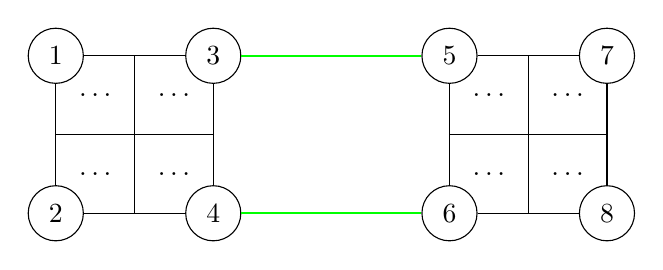
\begin{tikzpicture}[every node/.style={draw, circle, minimum size=0.7cm}]
        \node (1) at (0,2) {1};
        \node (2) at (0,0) {2};
        \node (3) at (2,2) {3};
        \node (4) at (2,0) {4};

        \node (5) at (5,2) {5};
        \node (6) at (5,0) {6};
        \node (7) at (7,2) {7};
        \node (8) at (7,0) {8};

        \draw (1) -- (2) -- (4) -- (3) -- (1);
        \draw (5) -- (7) -- (8) -- (6) -- (5);

        \draw[color=green, thick] (3) -- (5);
        \draw[color=green, thick] (4) -- (6);

        \draw (1,1) -- (1,0);
        \draw (1,1) -- (1,2);
        \draw (1,1) -- (0,1);
        \draw (1,1) -- (2,1);

        \draw (6,1) -- (5,1);
        \draw (6,1) -- (6,0);
        \draw (6,1) -- (6,2);
        \draw (6,1) -- (7,1);

        \node[draw=none] at (0.5,0.5) {\(\dots\)};
        \node[draw=none] at (1.5,0.5) {\(\dots\)};
        \node[draw=none] at (1.5,1.5) {\(\dots\)};
        \node[draw=none] at (0.5,1.5) {\(\dots\)};

        \node[draw=none] at (5.5,0.5) {\(\dots\)};
        \node[draw=none] at (6.5,0.5) {\(\dots\)};
        \node[draw=none] at (6.5,1.5) {\(\dots\)};
        \node[draw=none] at (5.5,1.5) {\(\dots\)};
    \end{tikzpicture}
    \caption{Simplified illustration of connectivity between components from adjacent hierarchical levels. The components (nodes 1-4 and 5-8) are connected only by the two green edges (3)--(5) and (4)--(6). Removing one endpoint from each edge (e.g., \{3, 6\}) forms a size-2 vertex separator, irrespective of component sizes.}
    \label{fig:nested_grid_connectivity_example}
\end{figure}
